\begin{Minutes}{}
%%\subtitle{}
%%\moderation{}
%%\minutetaker{}
\participant{Stephen Malina}
%%\missingExcused{}
%%\missingNoExcuse{}
\minutesdate{February 04, 2020}
%%\starttime{}
%%\endtime{}
%%\cc{}
\maketitle
\topic{Kipoi Uncertainty Estimates Cont.}
Managed to get mean, variance, and covariance estimates using all the stuff I've been working on this past week. In the process, I made two graphs which seem worth capturing here.

The first depicts predictive variance versus predictive mean with colors representing different sequences (each dot is for a maybe mutated variant of the sequence). As expected, predictive variance increases as predictions become more uncertain (become closer to 0.5).
\begin{figure}[t]
    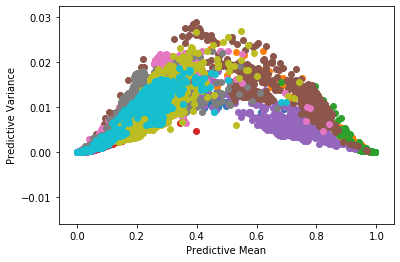
\includegraphics[width=0.8\linewidth]{figures/predictive_variance_vs_predictive_mean}
    \caption{Plot of predictive mean vs. predictive variance. Colors code for different sequences.}
\end{figure}
\end{Minutes}
